\begin{figure}
	\centering
	\pgfplotsset{every axis legend/.append style={
		at={(1.05,0.5)},
		anchor=west}}
	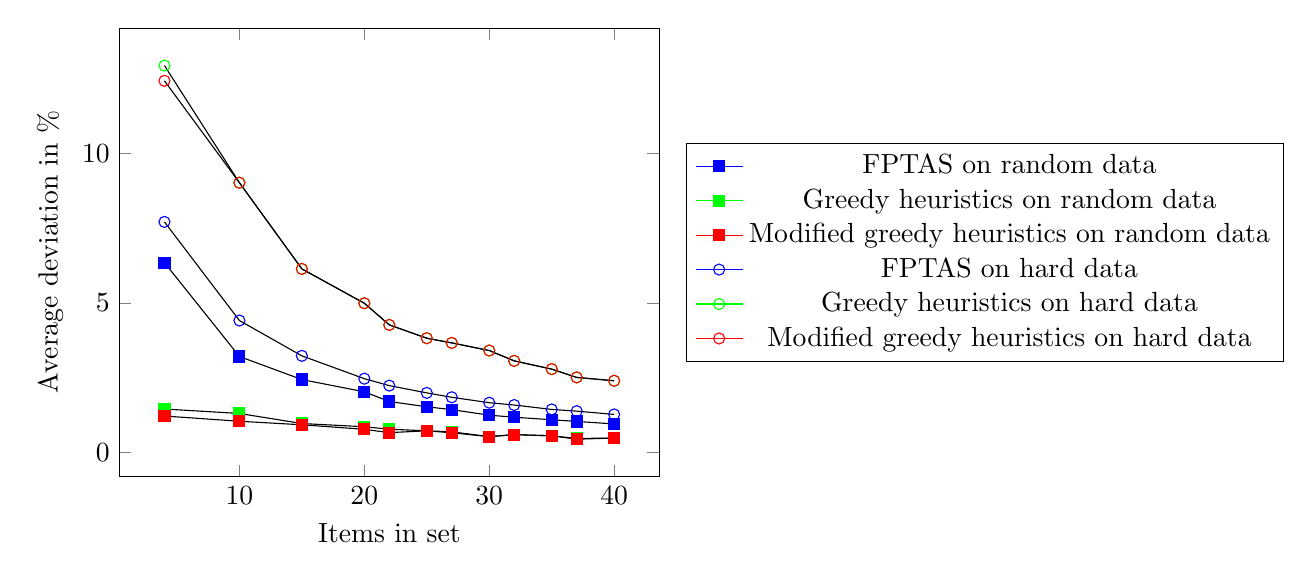
\begin{tikzpicture}
		\begin{axis}[
			xlabel=Items in set,
			ylabel=Average deviation in \%,
			scatter/classes={
				fptasN={mark=square*,blue},
				hungryN={mark=square*,green},
				singleN={mark=square*,red},
				fptasH={mark=o,blue},
				hungryH={mark=o,green},
				singleH={mark=o,red}
				}
			]
			\addplot[scatter,%
				scatter src=explicit symbolic]%
			table[meta=label] {
                x y label
                4 6.350120 fptasN
                10 3.210580 fptasN
                15 2.438080 fptasN
                20 2.029840 fptasN
                22 1.704882 fptasN
                25 1.528042 fptasN
                27 1.433396 fptasN
                30 1.247598 fptasN
                32 1.179112 fptasN
                35 1.093942 fptasN
                37 1.038356 fptasN
                40 .953716 fptasN
			};
			\addplot[scatter,%
				scatter src=explicit symbolic]%
			table[meta=label] {
				x y label
				4 1.453410 hungryN
                10 1.304166 hungryN
                15 .968396 hungryN
                20 .860422 hungryN
                22 .778518 hungryN
                25 .724522 hungryN
                27 .691782 hungryN
                30 .529006 hungryN
                32 .596280 hungryN
                35 .557696 hungryN
                37 .469084 hungryN
                40 .481640 hungryN
			};
			\addplot[scatter,%
				scatter src=explicit symbolic]%
			table[meta=label] {
                x y label
                4 1.219394 singleN
                10 1.043966 singleN
                15 .926256 singleN
                20 .774402 singleN
                22 .663398 singleN
                25 .724522 singleN
                27 .658822 singleN
                30 .529006 singleN
                32 .596280 singleN
                35 .557696 singleN
                37 .444584 singleN
                40 .481640 singleN
			};
			\addplot[scatter,%
				scatter src=explicit symbolic]%
			table[meta=label] {
				x y label
				4 7.711160 fptasH
                10 4.413000 fptasH
                15 3.231520 fptasH
                20 2.468120 fptasH
                22 2.235880 fptasH
                25 1.992836 fptasH
                27 1.845782 fptasH
                30 1.664936 fptasH
                32 1.586974 fptasH
                35 1.439758 fptasH
                37 1.382198 fptasH
                40 1.273106 fptasH
			};
			\addplot[scatter,%
				scatter src=explicit symbolic]%
			table[meta=label] {
				x y label
				4 12.939740 hungryH
                10 9.023060 hungryH
                15 6.139760 hungryH
                20 4.991380 hungryH
                22 4.266580 hungryH
                25 3.821660 hungryH
                27 3.664740 hungryH
                30 3.409840 hungryH
                32 3.063500 hungryH
                35 2.788140 hungryH
                37 2.510400 hungryH
                40 2.398320 hungryH
			};
			\addplot[scatter,%
				scatter src=explicit symbolic]%
			table[meta=label] {
                x y label
                4 12.430480 singleH
                10 9.023060 singleH
                15 6.139760 singleH
                20 4.991380 singleH
                22 4.266580 singleH
                25 3.821660 singleH
                27 3.664740 singleH
                30 3.409840 singleH
                32 3.063500 singleH
                35 2.788140 singleH
                37 2.510400 singleH
                40 2.398320 singleH
			};
			\addlegendentry{FPTAS on random data}
			\addlegendentry{Greedy heuristics on random data}
			\addlegendentry{Modified greedy heuristics on random data}
			\addlegendentry{FPTAS on hard data}
			\addlegendentry{Greedy heuristics on hard data}
			\addlegendentry{Modified greedy heuristics on hard data}
		\end{axis}
	\end{tikzpicture}
\caption{Average deviation in approximation algorithms}
\label{plot:deviation}
\end{figure}
